\documentclass[12pt]{article}
\usepackage{../../template}
\author{niceguy}
\title{Lecture 21}
\begin{document}
\maketitle

\section{Conservation Laws}

\subsection{Nomenclature}

$\vec{v}$ is the velocity vector, and $v = ||\vec{v}||$ is the fluid speed.

\subsection{Definitions}

\begin{defn}
	\emph{Volume Flow Rate} is the volume of fluid passing through a given surface per unit time. Its units are length cubed over time. Mathematically, it is
	$$\iint_A v_ndA$$
	where $v_n$ is the velocity component normal to the surface.
\end{defn}

\begin{defn}
	\emph{Mass Flow Rate} is defined similarly, represented mathematically as
	$$\iint_A \rho v_ndA$$
\end{defn}

\subsection{Conservation of Mass along a Streamtube}

Under steady and compressible conditions, mass should be constant, so
$$\dot{m}_1 = \dot{m}_2 \Rightarrow \rho_1v_1A_1 = \rho_2v_2A_2$$
Under steady and incompressible conditions, density is constant, which simplifies the above relation to
$$v_1A_1 = v_2A_2$$

\subsection{Conservation of Energy}

Imagine peeing/pooping. Kinetic energy is the difference between pressure energy and potential energy.

\subsection{Bernoulli Equation}

The \emph{Bernoulli Equation}, is valid in steady and incompressible flow with negligible frictional losses. Its derivation is as follows. \\
Consider a streamline. We use streamline coordinates with $\hat{s}$ in the direction of the steramline and $\hat{n}$ perpendicular to it.
$$\sum F_s = ma_s$$
Now, forces come from pressure and self weight, i.e.
$$\sum F_s = W_s + \sum F_{p,s} = -\rho g dAds\sin\theta + pdA - (p+dp)dA = -\rho gdAdz - dpdA$$
Using the chain rule,
$$a_s = \frac{dv_s}{ds}\frac{ds}{dt} = v_s\frac{dv_s}{ds}$$
Mass is given by
$$m = \rho dAds$$
Equating both sides,
\begin{align*}
	-\rho gdAdz - dpdA &= \rho dAdsv_s\frac{dv_s}{ds} \\
	-gdz - \frac{1}{\rho}dp &= dsv_s\frac{dv_s}{ds} \\
	v_sdv_s + gdz + \frac{1}{\rho}dp &= 0
\end{align*}
This gives the \emph{Euler's Equation}. If incompressible flow is assumed, both sides can be integrated to give
$$\frac{v_s^2}{2} + gz + \frac{p}{\rho} = C$$
where $C$ is an arbitrary constant. This is the \emph{Bernoulli Equation}. Note that it has units of energy per mass. The constant is the same at any point along the same strealine, meaning
$$\frac{v_1}{2} + gz_1 + \frac{p_1}{\rho} = \frac{v_2}{2} + gz_2 + \frac{p_2}{\rho}$$
In fact, for a stationary fluid,
$$gdz + \frac{1}{\rho}dp = 0$$
If the fluid is incompressible,
$$gz + \frac{p}{\rho} = C$$
or
$$p_1-p_2 = \rho g(z_2-z_1)$$

\subsection{Different Pressures}
Based on the Bernoulli Equation, multiply by $\rho$, we have
$$p + \frac{\rho v^2}{2} + \rho gz = P_T$$
where the terms are called static pressure, dynamic pressure, hydrostatic pressure and total pressure respectively.

\begin{figure}
	\centering
	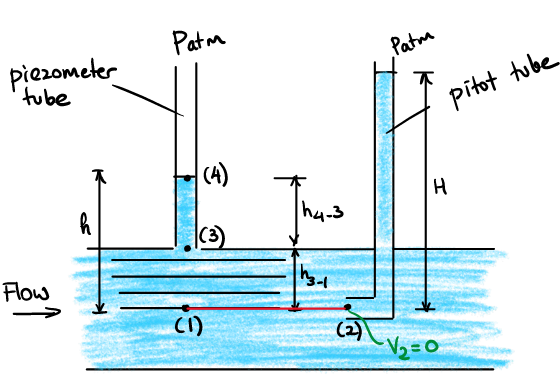
\includegraphics[width=0.7\textwidth]{tubes.png}
	\caption{Illustration of Different Pressures}
	\label{tubes}
\end{figure}

The static pressure can be measured with a piezometer tube, and the dynamic pressure can be found using a pitot tube (Fig~\ref{tubes}). The pitot tube measures the stagnation pressure, which is defined as the sum of the static and dynamic pressures.

\subsection{Limitation on the Use of the Bernoulli Equation}

\begin{itemize}
	\item Steady Flow
	\item Incompressible Flow
	\item Frictionless Flow
	\item Flow along a Streamline
	\item No shaft work between points 1 and 2
	\item No heat transfer between points 1 and 2
\end{itemize}

\begin{ex}
	A large tank open to the atmosphere is filled with water to a height of 5m from the outliet tap. A tap near the bottom of the atank is now opened, and wtaer flows out from the smooth and rounded outlet. Determine the water velocity at the outlet.
	\begin{align*}
		\frac{p_1}{\rho} + \frac{v_1^2}{2} + gz_1 &= \frac{p_2}{\rho} + \frac{v_2}{2} + gz_2 \\
		5g &= \frac{v_2^2}{2} \\
		v_2 &= \sqrt{10g} \\
		    &= 10
	\end{align*}
\end{ex}

\section{Flowrate Measurement}

A common way to measure the flowrate through a pipe is to place some type of restriction within the pipe and to measure the pressure difference between the sections before and after the restriction. As height is approximately constant, the equation simplifies to
$$p_1 + \frac{\rho v_1^2}{2} = p_2 + \frac{\rho v_2^2}{2}$$
Combining this with
$$v_1A_1 = v_2A_2$$
we have
$$v_2 = \sqrt{\frac{2(p_1-p_2)}{\rho\left(1-\left(\frac{A_2}{A_1}\right)^2\right)}}$$

\section{Momentum}

\subsection{Control Volume Approach vs System Approach}

The Control Volume Approach (Eulerian) observes the particles travelling through a fixed volume. The System Approach (Lagrangian) defines a moving system of the same particles.

\section{Reynolds Transport Theorem}

$$B = mb$$
where $B$ is a parameter proportional with the mass of the fluid, and $b$ is the parameter per unit mass.

\begin{ex}
	Time rate of change for a system and a control volume.
	$$\frac{dB_\mathrm{sys}}{dt} = \frac{dm_\mathrm{sys}}{dt} = 0$$
	but
	$$\frac{dB_\mathrm{cv}}{dt} = \frac{dm_\mathrm{cv}}{dt} < 0$$
	They are different!
\end{ex}
\end{document}
